
\subsubsection{Multi-Layer Perceptron}

Next, the \texttt{neuralnet} function from the \texttt{mlp} package is used to fit a multi-layer perceptron network to the earthquake data.  After pre-processing to split the data, the network architectue is defined as a three-layer network with 5 neurons in each hidden layer.  The function uses resilient backpropagation by default and sigmoid activation between layers.

\begin{Shaded}
\begin{Highlighting}[]
\FunctionTok{set.seed}\NormalTok{(}\DecValTok{4723}\NormalTok{)}

\CommentTok{\#shuffle the data}
\NormalTok{df }\OtherTok{\textless{}{-}}\NormalTok{ earthquakes\_log[}\FunctionTok{sample}\NormalTok{(}\FunctionTok{nrow}\NormalTok{(earthquakes\_log)), ]}

\CommentTok{\#Extract 70\% of data into train set and the remaining 30\% in test set}
\NormalTok{train\_test\_split }\OtherTok{\textless{}{-}} \FloatTok{0.7} \SpecialCharTok{*} \FunctionTok{nrow}\NormalTok{(df)}
\NormalTok{train }\OtherTok{\textless{}{-}}\NormalTok{ df[}\DecValTok{1}\SpecialCharTok{:}\NormalTok{train\_test\_split,]}
\NormalTok{test }\OtherTok{\textless{}{-}}\NormalTok{ df[(train\_test\_split}\SpecialCharTok{+}\DecValTok{1}\NormalTok{)}\SpecialCharTok{:} \FunctionTok{nrow}\NormalTok{(df),]}

\NormalTok{mlp }\OtherTok{\textless{}{-}} \FunctionTok{neuralnet}\NormalTok{(freqc }\SpecialCharTok{\textasciitilde{}}\NormalTok{ mag,}
                 \AttributeTok{stepmax =} \FloatTok{1e+06}\NormalTok{,}
                 \AttributeTok{data =}\NormalTok{ train,}
                 \AttributeTok{hidden =} \FunctionTok{c}\NormalTok{(}\DecValTok{5}\NormalTok{,}\DecValTok{5}\NormalTok{))}

\CommentTok{\#prediction for magnitude 9.1}
\NormalTok{p }\OtherTok{\textless{}{-}} \FunctionTok{predict}\NormalTok{(mlp, }\AttributeTok{newdata =} \FunctionTok{data.frame}\NormalTok{(}\AttributeTok{mag =} \FloatTok{9.1}\NormalTok{))}
\DecValTok{1}\SpecialCharTok{/}\DecValTok{10}\SpecialCharTok{\^{}}\NormalTok{p}
\end{Highlighting}
\end{Shaded}

\begin{verbatim}
##          [,1]
## [1,] 3212.887
\end{verbatim}

Using this neural network model, the expected frequency of a magnitude
9.1 earthquake would be one every 3,212.89 years.  That's less frequent than the base linear model from before, and more frequent than the second order polynomial model that accounted for the curvature of the data.  Still it may not be enough to convince the Fukushima engineering officials to build a stronger reactor.  A plot of the data is shown below:

\begin{figure}[H]
    \center
    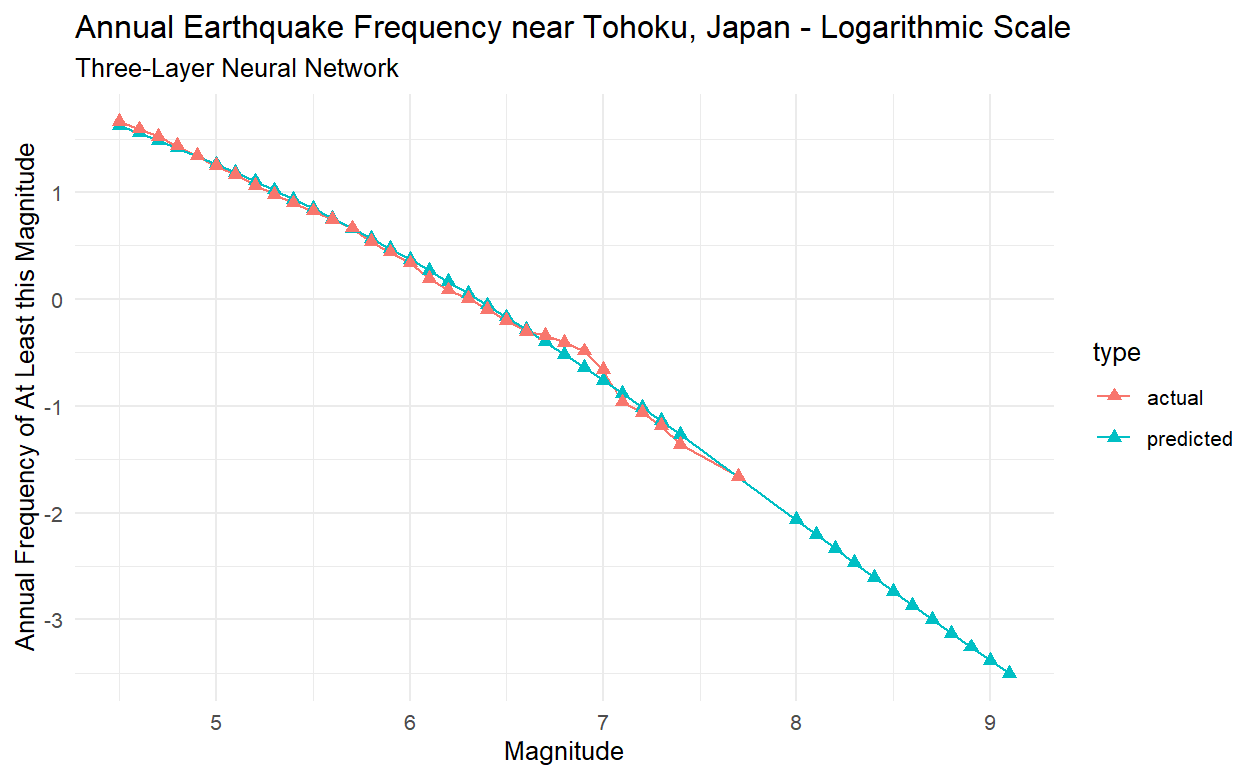
\includegraphics[width=0.8\linewidth]{Figures/tohoku_logscale_mlp.png}
   % \vspace{-10pt}
    \caption{\footnotesize{Actual data points plotted with MLP-predicted values for all data points, with appended predicted magnitudes for sequential series of magnitude 8.0 - 9.1 by 0.1}}
    \label{tohoku_mlp}
\end{figure}


\subsubsection{Capacity Simulation for Neural Network}

Adding more neurons or more layers to a neural network can increase its capacity.  The code below builds different networks to answer the same question in predicting Tohoku earthquake frequencies.  For each model, the test error is calculated by sums of squares.  Three networks are made, each with one more layer than the previous and each with 5 neurons per hidden layer.

\begin{Shaded}
\begin{Highlighting}[]
\FunctionTok{set.seed}\NormalTok{(}\DecValTok{4723}\NormalTok{)}
\CommentTok{\#{-}{-}{-}one hidden layer{-}{-}{-}}
\NormalTok{mlp }\OtherTok{\textless{}{-}} \FunctionTok{neuralnet}\NormalTok{(freqc }\SpecialCharTok{\textasciitilde{}}\NormalTok{ mag,}
                 \AttributeTok{stepmax =} \FloatTok{1e+06}\NormalTok{,}
                 \AttributeTok{data =}\NormalTok{ train,}
                 \AttributeTok{hidden =} \FunctionTok{c}\NormalTok{(}\DecValTok{5}\NormalTok{))}

\CommentTok{\#predictions on test data}
\NormalTok{pps }\OtherTok{\textless{}{-}} \FunctionTok{predict}\NormalTok{(mlp, }\AttributeTok{newdata =} \FunctionTok{data.frame}\NormalTok{(}\AttributeTok{mag =}\NormalTok{ test}\SpecialCharTok{$}\NormalTok{mag))}

\CommentTok{\#SSE to get test error}
\NormalTok{TestErr1 }\OtherTok{\textless{}{-}} \FunctionTok{sum}\NormalTok{((pps }\SpecialCharTok{{-}}\NormalTok{ test}\SpecialCharTok{$}\NormalTok{freqc)}\SpecialCharTok{\^{}}\DecValTok{2}\NormalTok{)}
\NormalTok{TrainErr1 }\OtherTok{\textless{}{-}}\NormalTok{ mlp}\SpecialCharTok{$}\NormalTok{result.matrix[}\DecValTok{1}\NormalTok{,]}

\FunctionTok{set.seed}\NormalTok{(}\DecValTok{4723}\NormalTok{)}
\CommentTok{\#{-}{-}{-}two hidden layers{-}{-}{-}}
\NormalTok{mlp }\OtherTok{\textless{}{-}} \FunctionTok{neuralnet}\NormalTok{(freqc }\SpecialCharTok{\textasciitilde{}}\NormalTok{ mag,}
                 \AttributeTok{stepmax =} \FloatTok{1e+06}\NormalTok{,}
                 \AttributeTok{data =}\NormalTok{ train,}
                 \AttributeTok{hidden =} \FunctionTok{c}\NormalTok{(}\DecValTok{5}\NormalTok{,}\DecValTok{5}\NormalTok{))}

\CommentTok{\#predictions on test data}
\NormalTok{pps }\OtherTok{\textless{}{-}} \FunctionTok{predict}\NormalTok{(mlp, }\AttributeTok{newdata =} \FunctionTok{data.frame}\NormalTok{(}\AttributeTok{mag =}\NormalTok{ test}\SpecialCharTok{$}\NormalTok{mag))}

\CommentTok{\#SSE to get test error}
\NormalTok{TestErr2 }\OtherTok{\textless{}{-}} \FunctionTok{sum}\NormalTok{((pps }\SpecialCharTok{{-}}\NormalTok{ test}\SpecialCharTok{$}\NormalTok{freqc)}\SpecialCharTok{\^{}}\DecValTok{2}\NormalTok{)}
\NormalTok{TrainErr2 }\OtherTok{\textless{}{-}}\NormalTok{ mlp}\SpecialCharTok{$}\NormalTok{result.matrix[}\DecValTok{1}\NormalTok{,]}

\FunctionTok{set.seed}\NormalTok{(}\DecValTok{4723}\NormalTok{)}
\CommentTok{\#{-}{-}{-}three hidden layers{-}{-}{-}}
\NormalTok{mlp }\OtherTok{\textless{}{-}} \FunctionTok{neuralnet}\NormalTok{(freqc }\SpecialCharTok{\textasciitilde{}}\NormalTok{ mag,}
                 \AttributeTok{stepmax =} \FloatTok{1e+06}\NormalTok{,}
                 \AttributeTok{data =}\NormalTok{ train,}
                 \AttributeTok{hidden =} \FunctionTok{c}\NormalTok{(}\DecValTok{5}\NormalTok{,}\DecValTok{5}\NormalTok{,}\DecValTok{5}\NormalTok{))}

\CommentTok{\#predictions on test data}
\NormalTok{pps }\OtherTok{\textless{}{-}} \FunctionTok{predict}\NormalTok{(mlp, }\AttributeTok{newdata =} \FunctionTok{data.frame}\NormalTok{(}\AttributeTok{mag =}\NormalTok{ test}\SpecialCharTok{$}\NormalTok{mag))}

\CommentTok{\#MSE to get test error}
\NormalTok{TestErr3 }\OtherTok{\textless{}{-}} \FunctionTok{sum}\NormalTok{((pps }\SpecialCharTok{{-}}\NormalTok{ test}\SpecialCharTok{$}\NormalTok{freqc)}\SpecialCharTok{\^{}}\DecValTok{2}\NormalTok{)}
\NormalTok{TrainErr3 }\OtherTok{\textless{}{-}}\NormalTok{ mlp}\SpecialCharTok{$}\NormalTok{result.matrix[}\DecValTok{1}\NormalTok{,]}

\CommentTok{\#View results}
\NormalTok{TestError }\OtherTok{\textless{}{-}} \FunctionTok{cbind}\NormalTok{(TestErr1,TestErr2,TestErr3)[}\DecValTok{1}\SpecialCharTok{:}\DecValTok{3}\NormalTok{]}
\NormalTok{TrainError }\OtherTok{\textless{}{-}} \FunctionTok{cbind}\NormalTok{(TrainErr1, TrainErr2, TrainErr3)[}\DecValTok{1}\SpecialCharTok{:}\DecValTok{3}\NormalTok{]}
\NormalTok{GeneralizationGap }\OtherTok{\textless{}{-}}\NormalTok{ TrainError }\SpecialCharTok{{-}}\NormalTok{ TestError}

\FunctionTok{data.frame}\NormalTok{(}\FunctionTok{rbind}\NormalTok{(TestError,TrainError,GeneralizationGap))}
\end{Highlighting}
\end{Shaded}

\begin{verbatim}
##                            X1          X2         X3
## TestError         0.009838334 0.008655795 0.01114061
## TrainError        0.038023503 0.017808021 0.02909132
## GeneralizationGap 0.028185169 0.009152226 0.01795071
\end{verbatim}

% latex table generated in R 4.2.2 by xtable 1.8-4 package
% Thu Apr 27 13:43:54 2023
\begin{table}[ht]
\centering
\begin{tabular}{rrrr}
  \hline
 & 1 Hidden Layer & 2 Hidden Layers & 3 Hidden Layers \\ 
  \hline
Test Error & 0.0098383338 & 0.0086557953 & 0.0111406131 \\ 
  Train Error & 0.0380235026 & 0.0178080209 & 0.0290913220 \\ 
  Generalization Gap & 0.0281851688 & 0.0091522255 & 0.0179507089 \\ 
   \hline
\end{tabular}
\end{table}

The table above shows error measurements for a network with one, with two, and with three hidden layers.  The \textit{generalization gap}, which is a measure of difference between the two errors, is minimized for the network with two hidden layers.  That this value increases moving from a network with two to three hidden layers is indicative that the three-layer model is overfit.  Based on this table, the model with two hidden layers used above is the optimal fit.  However, this model is devoid of any regularization technique.  In a later section, the same example will be revisited using \textit{weight decay} in which parameters $\alpha$ and $\beta$ are determined from a Bayesian approach.  In the meantime, this thesis will summarize some important and methods of Bayesian Statistics.